\documentclass{llncs}
\usepackage{amsmath,amsfonts,amssymb}
\usepackage{graphicx}
\usepackage{makeidx}  % allows for indexgeneration
\begin{document}

\title{Simulation of Tsunami impact upon Coastline}

\titlerunning{Tsunami simulation}

\author{Konstantinos Moustakas\inst{1} \and Aristotelis Spathis-Papadiotis\inst{1}}
\authorrunning{Konstantinos Moustakas et al.} % abbreviated author list (for running head)

%%%% list of authors for the TOC (use if author list has to be modified)
\tocauthor{Konstantinos Moustakas, Aristotelis Spathis-Papadiotis}

\institute{Electrical and Computer Engineering Department\\
  University of Patras, Patra, Greece\\
  \email{moustakas@upatras.gr}}

\maketitle

\begin{abstract}
  Presented in this paper is a simulation of a tsunami impact upon an urban
  coastline. Emphasis was given to the conservation of momentum during the simulation, as
  its distribution in space and time is the main factor of the wave's effects on the
  coastline. Due to this, a hybrid simulation method was adopted, based on the Smoothed
  Particle Hydrodynamics method, enriched with geometric constraints and rigid body
  interactions. The implementation is the result of cooperation between the Bullet physics
  engine and a custom SPH engine, which successively process the dynamic state of the
  fluid at every timestep of the simulation. Furthermore, in order to achieve better
  performance a custom data structure (LP grid) was developed for the optimization of
  locality in data storage and minimization of access time. Simulation data is exported to
  VTK files to allow interactive processing and visualization with the aid of specialized
  programs (like ParaView\texttrademark). \keywords{Fluid simulation, tsunami, SPH,
    tsunami-coastline interaction, force visualization}
\end{abstract}

\section{Introduction}

\paragraph{} Simulations of natural phenomena are a precious tool for analysis and
understanding of the processes behind them as well as the implications of
those. Especially fluid dynamics is one of the fields most benefitted by the explosion of
high performance parallel computing architectures of the last years. Tsunamis are one of
the most devastating natural disasters, with much attention drawn to them lately,
especially after the 2004 Indian Ocean tsunami and the 2011 T\={o}hoku earthquake and
tsunami, two of the largest incidents of modern history. Multiscale modelling of tsunami
generation, propagation and impact is a trending research area as respective simulations
give valuable insights into the underlying mechanisms and relations between the various
stages of an unfolding tsunami incident, while also facilitating the assessment of
potential hazard it poses upon impact on a coastline.

\paragraph{} A tsunami is a series of waves in a water body caused by an impulsive
disturbance that vertically displaces a large volume of water. Tsunamis are generated by
earthquakes, volcanic eruptions, landslides and other such events which have the potential
to transmit a huge amount of mechanical energy to a water column. At large scales, tsunami
propagation in the ocean is usually modelled through various versions of the Shallow Water
Equations, derived from the Navier-Stokes equations in the case where the horizontal
length scale is much greater than the vertical one. Conversely, simulations of tsunami
impact is usually carried out using other methods, since complex dynamics must be taken
into account. One of the most used methods for simulating complex flows with multiple
boundary interactions is Smoothed Particle Hydrodynamics, initially proposed in the 1970s
for treatment of compressible flows in astrophysical problems. Since then, it has been
applied to a wide variety of fields such as aerodynamics, geology, computer graphics and
engineering with exceptional results. In our simulation, emphasis was given to the
conservation of momentum and its distribution upon the coastline during the tsunami
impact. Therefore, we adopted SPH as our method of choice due to its unparalleled
advantages it offers, relating to its properties as lagrangian method.

\section{SPH Methodology}

\paragraph{} SPH is a lagrangian fluid simulation method, based on the discretization of
the fluid into particles which serve as interpolation points for the estimation of fluid
properties in space. Advantages of this method include the exact treatment of advection,
the natural way of dealing with special interface interactions, the inherent conservation
of significant quantities (mass, momentum, energy) and the self-adaptivity of
computational load to the fluid location and state in the flow domain. Starting from the
identity:
\begin{equation*}
  f(\vec{r}) = \int_Vf(\vec{x}) \delta(\vec{r} - \vec{x}) d\vec{x},
\end{equation*}
where $\delta(\vec{r})$ the Dirac delta function and $\vec{x} \in V$, we can obtain a more
general interpolation rule by substituting $\delta(\vec{r})$ with a smoothing kernel
$W(\vec{r}, h)$:
\begin{equation*}
  \label{eq:c-approx}
  f(\vec{r}) \approx \int_V f(\vec{x}) W(\vec{r}-\vec{x}, h) d\vec{x}
\end{equation*}
whose limit when $h\to0$ approaches the delta fucntion and is normalized to unity:
\begin{equation*}
  \label{eq:kernel-properties}
  \lim_{h\to0}W(\vec{r}, h) = \delta(\vec{r})\ \ \
  \text{and}\ \ \
  \int_VW(\vec{r}, h) d\vec{x} = 1
\end{equation*}
The smoothing radius $h$ serves as a cutoff radius in the smoothing process, as particles
beyond that distance have no contribution to the sum, i.e. $W(r,h) = 0$ when $r>h$. For
the discrete case, where $f$ is discretized to particles with density $\rho$ and mass $m$,
the weighting ratio $m/\rho$ can be used to construct a weighted sum interpolant for any
field $A$:
\begin{equation}
  \label{eq:d-approx}
  A(\vec{r}) = \sum_i \frac{m_i}{\rho_i} A(\vec{r}_i) W(\vec{r}-\vec{x}_i, h)
\end{equation}
which lies at the heart of SPH formulation. According to this, the gradient can be
computed by the following approximation:
\begin{equation}
  \label{eq:d-grad}
  \nabla A(\vec{r}) = \sum_i \frac{m_i}{\rho_i} A(\vec{r}_i) \nabla W(\vec{r} - \vec{x}_i, h)
\end{equation}
The obvious advantage of this is the exclusive dependence on the smoothing kernel
gradient, which can be precomputed for sensible kernel choices. However, this formula can
lead to unsymmetric pair forces, compromising the conservation of linear and angular
momentum of the system. To symmetrize these forces depending on gradients (like those
originating from pressure differences), we can use the product rule:
\begin{equation*}
  \label{eq:grad-identity}
  \nabla \left( \frac{P}{\rho} \right) =
  \frac{\nabla P}{\rho}-
  \frac{P}{\rho^2} \nabla \rho
  \hspace{10pt} \Leftrightarrow \hspace{10pt}
  \nabla P = \rho \left[ \frac{P}{\rho^2} \nabla \rho + \nabla \left( \frac{P}{\rho}
    \right) \right]
\end{equation*}
to obtain an alternative approximation of gradient
\begin{align}
  \label{eq:grad-est}
  \nabla P & = \rho \left[ \frac{P}{\rho^2} \sum_i \frac{m_i}{\rho_i} \rho \nabla
             W(\vec{r}-\vec{r}_i, h)
             +
             \sum_i \frac{m_i}{\rho_i} \frac{P_i}{\rho_i} \nabla W(\vec{r}-\vec{r}_i, h)
             \right] \nonumber \\
           & = \rho \sum_i m_i \left(\frac{P}{\rho^2} + \frac{P_i}{\rho_i} \right)
             \nabla W(\vec{r}-\vec{r}_i, h)
\end{align}
which is antisymmetric for all interacting particle pairs. Viscosity forces on the other
hand, are proportional to the laplacian of the velocity field:
\begin{equation}
  \label{eq:lapl-est}
  \nabla^2\vec{v} = \sum_i \frac{m_i}{\rho_i} (\vec{v}_i - \vec{v}) \nabla^2
  W(\vec{r}-\vec{r}_i, h)
\end{equation}
and are always antisymmetric, since they depend on velocity difference
$\vec{v}_i - \vec{v}$ between particles.  In each timestep of the simulation, the density
of all particles is first computed according to equation \ref{eq:d-grad}, as it depends
only on the relative position of those. The pressure at each particle location is then
obtained from its respective density through an equation of state. Subsequently, the
pressure and viscosity forces are computed from the particle data and integrated back into
the position and velocity of the particles.

\section{Implementation}

\paragraph{} Each simulation under our implementation consists of two elements, the
coastline terrain (static) and the tsunami wave (dynamic). For the simulation setup,
terrain is imported from a suitable 3D geometry definition file format, the initial
conditions of the impacting wave (position and velocity) are configured, and the desired
discretization resolution for the fluid is set. From these conditions, the terrain and
fluid are initialized, and key parameters are computed. Terrain geometry is scaled by a
user-supplied factor and docked to the origin of coordinates, while fluid particles are
initially placed into an Hexagonal Close-Packed lattice, to achieve the densest possible
packing and symmetry:
\begin{equation}
  \label{eq:hcp}
  [x, y, z] = \left[ 2i+[(j+k) \bmod 2], \sqrt{3}[j + \frac{1}{3} (k \bmod 2)],
    \frac{2\sqrt{6}}{3} k \right] r
\end{equation}
In this configuration, the smoothing radius $h$ is computed such that each particle has
approximately 50 neighbours (following the empirical rule established in the
literature). The timestep is determined according to the Courant-Friedrichs-Lewy
criterion:
\begin{equation}
  \label{eq:cfl}
  \delta t_{\text{CFL}} = C \frac {\delta x}{v_{\text{max}}},
\end{equation}
for values of Courant number $C\approx0.5$ with characteristic length $\delta x$ equal to
the effective particle radius and maximum velocity $v_{\text{max}}$ determined by the
maximum potential energy in the initial configuration. Following standard practice, we
used three different smoothing kernels for density, pressure gradient and velocity
laplacian computation:
\begin{equation}
  \label{eq:poly6}
  W_{\text{poly6}}(r, h) = \frac{315}{64 \pi h^9}
  \begin{cases}
    (h^2 - r^2)^3 & 0 \leq r \leq h\\
    0 & \text{otherwise}
  \end{cases}
\end{equation}
\begin{equation}
  \label{eq:spiky}
  W_{\text{spiky}}(r, h) = \frac{15}{\pi h^6}
  \begin{cases}
    (h - r)^3 & 0 \leq r \leq h\\
    0 & \text{otherwise}
  \end{cases}
\end{equation}
\begin{equation*}
  \label{eq:spiky-gradient}
  \nabla W_{\text{spiky}}(r, h) = \frac{-45}{\pi h^6} (h-r)^2
\end{equation*}
\begin{equation}
  \label{eq:viscosity}
  W_{\text{viscosity}}(r, h) = \frac{15}{2 \pi h^3}
  \begin{cases}
    - \frac{r^3}{2h^3} + \frac{r^2}{h^2} + \frac{h}{2r} - 1 & 0 \leq r \leq h\\
    0 & \text{otherwise},
  \end{cases}\\
\end{equation}
\begin{equation*}
  \label{eq:viscosity-laplacian}
  \nabla^2 W_{\text{viscosity}}(r, h) = \frac{45}{\pi h^6} (h-r)
\end{equation*}

\paragraph{} For the computation of the pressure from the estimated fluid density, the
ideal gas equation of state is used:
\begin{equation}
  \label{eq:ideal-state}
  P = k(\rho - \rho_0),
\end{equation}
according to which the pressure is proportional to the difference of the current from the
rest density. The major problem with this equation of state are the compressibility issues
that have been shown to exist in simulations using it. A frequently proposed solution is
to replace the above with the Tait equation of state:
\begin{equation}
  \label{eq:tait-state}
  P = B \left( \left( \frac{\rho}{\rho_0} \right)^\gamma - 1 \right),
\end{equation}
where usually $\gamma=7$ and $B$ a proportionality constant controlling the tolerance to
density fluctuations. This equation is much more punishing on density fluctuations away
from the rest density, therefore requiring significantly smaller timesteps to ensure
stability. Here we follow a different approach, inspired by Position Based Dynamics, in
which particles are represented by spherical rigid bodies. The most important advantage of
this technique is the elegant handling of boundary, undersampled and degenerate fluid
regions that tend to arise very frequently in simulations of free flows. The adoption of
this approach allows to treat boundary collisions in a simple manner, while naturally
enforcing incompressibility near boundaries and free surfaces. In these regions,
estimators fall short to describe the actual flow regime due to neighbour particle
shortage. This undersampling creates the need for correction procedures, usually involving
ghost/boundary particles, to avoid pressure instabilities, particle clustering and other
artifacts. On the contrary, no such method is necessary under our representation, where
degenerative cases are handled through geometric constraints thus selectively preventing
unreliable estimations from affecting the flow.

\paragraph{} The Bullet physics engine is used to handle the rigid body dynamics. The
simulation domain is divided by a regular grid of spacing equal to the smoothing radius
into cells containing the fluid particles, which are generated as Bullet objects and
stored in a custom cell list data structure consisting of three vectors. Particles are
then accessed by following pointers through those vectors in order, with the first
encoding the 3D to linear locality preserving mapping of cells on the second, and the
second pointing at first of the cell's particles which are continuously stored on the
third, a dynamic sliding vector. This data structure allows for quick neighbour search,
interaction scanning, exploitation of access patterns of the SPH algorithm and fast,
in-place update. Simulation is following the Bullet framework, with the SPH code being
embedded as an internal timestep tick callback function. We took advantage of the Bullet
infrastructure to extract detailed information about the collisions between fluid and
terrain regarding the resulting impulse, time, and location. Impulse and particle data are
then written to multiple VTK files per frame. Samples of the smoothed color field (common
name in the literature for the field having the value 1 at particle locations and 0
everywhere else) on the regular cell lattice are also exported, which are then used to
reconstruct the fluid surface as an isosurface of that field. At the end of the simulation
a cumulative impulse heatmap along with the scaled and docked terrain model are also
provided.

\section{Results}
\paragraph{} Multiple simulations were carried out using different models of urban
coastline, in order to gain a significant and diverse dataset of impulses exerted over the
duration of the impact. Tsunamis are vastly different from the usual wind-induced sea
waves in that they have far longer wavelength and carry much greater total energy,
appearing as a rapidly rising tide instead of a breaking waves. Accounting for these
facts, we chose to represent the tsunami wave as a water volume invading the coastline
with an initial velocity.
% \begin{figure}
%   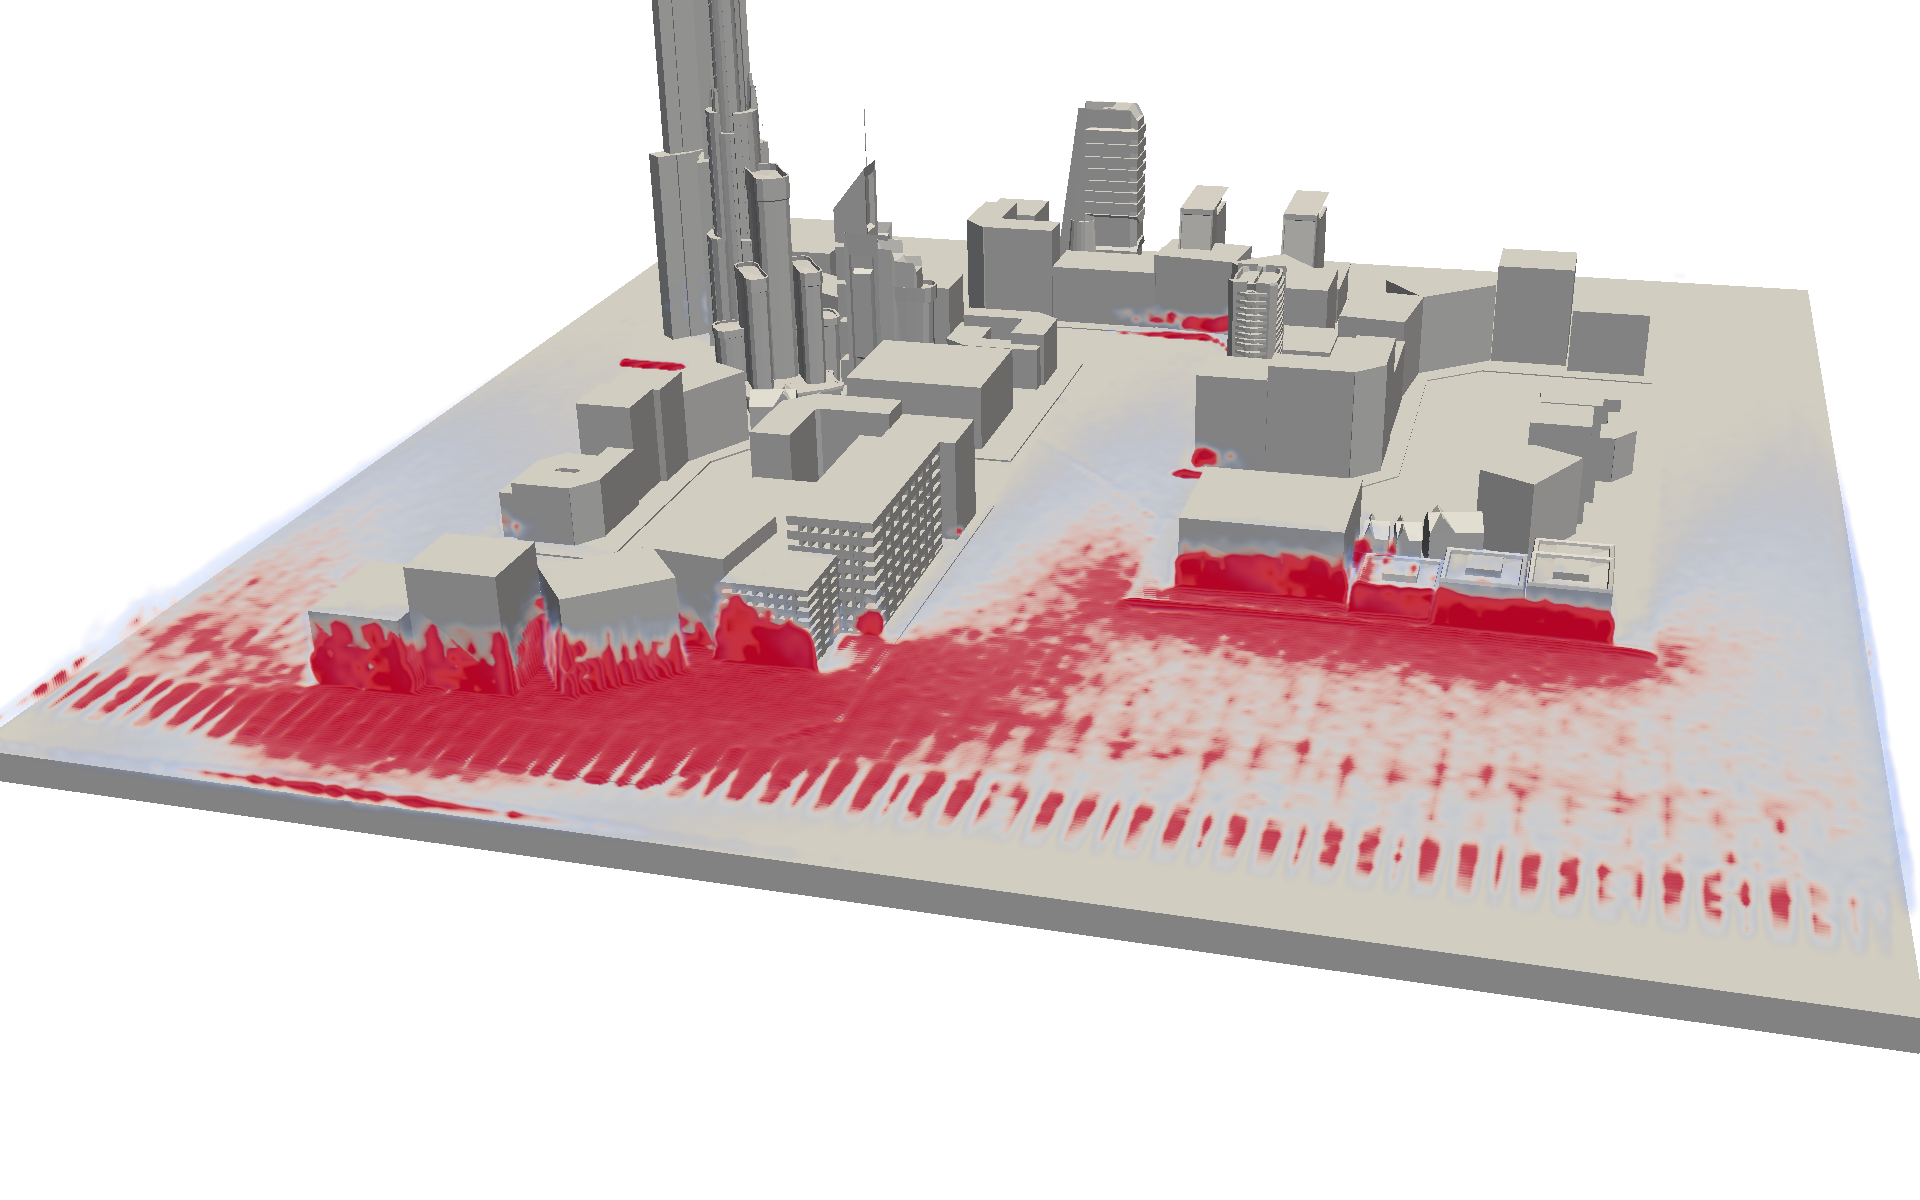
\includegraphics[width=\textwidth]{../report/figures/impulse-heatmap-0.png}
%   \caption{Impulse heatmap on a coastline}
% \end{figure}


\section{Future Work}

% ---- Bibliography ----
\begin{thebibliography}{0}

  % \bibitem {clar:eke}
  %   Clarke, F., Ekeland, I.:
  %   Nonlinear oscillations and
  %   boundary-value problems for Hamiltonian systems.
  %   Arch. Rat. Mech. Anal. 78, 315--333 (1982)

  % \bibitem {clar:eke:2}
  %   Clarke, F., Ekeland, I.:
  %   Solutions p\'{e}riodiques, du
  %   p\'{e}riode donn\'{e}e, des \'{e}quations hamiltoniennes.
  %   Note CRAS Paris 287, 1013--1015 (1978)

  % \bibitem {mich:tar}
  %   Michalek, R., Tarantello, G.:
  %   Subharmonic solutions with prescribed minimal
  %   period for nonautonomous Hamiltonian systems.
  %   J. Diff. Eq. 72, 28--55 (1988)

  % \bibitem {tar}
  %   Tarantello, G.:
  %   Subharmonic solutions for Hamiltonian
  %   systems via a $\bbbz_{p}$ pseudoindex theory.
  %   Annali di Matematica Pura (to appear)

  % \bibitem {rab}
  %   Rabinowitz, P.:
  %   On subharmonic solutions of a Hamiltonian system.
  %   Comm. Pure Appl. Math. 33, 609--633 (1980)

\end{thebibliography}

\end{document}

%%% Local Variables:
%%% mode: latex
%%% TeX-master: t
%%% End:
